\setcounter{page}{1}

\section{Introducción}
    NAT, o Traducción de Direcciones de Red, es un proceso que modifica la información de dirección de red en la cabecera IP de los paquetes mientras estos se transmiten a través de un dispositivo de enrutamiento de tráfico (\cite{ormeci25}). 
    
    En términos sencillos, NAT permite que varios dispositivos en una red local, como una casa u oficina, se conecten a Internet utilizando una sola dirección IP pública. Esto se logra mediante la traducción de las direcciones IP privadas internas de los dispositivos a una dirección IP pública antes de que los paquetes se envíen a la red externa. Es importante destacar que NAT no es solo una herramienta de gestión de red, sino que también puede considerarse una característica de seguridad. Al ocultar las direcciones IP internas, NAT dificulta que los usuarios externos se conecten directamente a los dispositivos de la red interna, a menos que se haya configurado una asignación específica. Esto ayuda a prevenir el tráfico entrante no solicitado y reduce el riesgo de ataques (\cite{cisco23}).
    Existen diferentes tipos de NAT, cada uno con características y aplicaciones específicas:

    \begin{itemize}
        \item \textbf{NAT estático:} Asigna una dirección IP privada a una dirección IP pública fija. Esto permite que un dispositivo interno siempre se vea en Internet con la misma dirección IP.
        \item \textbf{NAT dinámico:} A diferencia del NAT estático, el NAT dinámico utiliza un conjunto de direcciones IP públicas y las asigna a los dispositivos internos según el orden de llegada. Esto permite que varios dispositivos compartan un grupo más pequeño de direcciones IP públicas, lo que lo hace más escalable. Sin embargo, la asignación entre las direcciones IP privadas y públicas no es permanente y puede cambiar con cada sesión.
        \item \textbf{NAT de traducción de puertos (PAT):} También conocido como NAT con sobrecarga, PAT permite que múltiples dispositivos compartan una única dirección IP pública mediante la traducción de direcciones IP y puertos. Cada dispositivo recibe un puerto único en la dirección IP pública, lo que permite que el router distinga el tráfico de cada dispositivo. PAT es el tipo de NAT más utilizado en redes domésticas y pequeñas empresas, ya que permite que muchos dispositivos se conecten a Internet con una sola dirección IP pública proporcionada por el ISP.
    \end{itemize}

    Un ISP, o Proveedor de Servicios de Internet, es una empresa que proporciona acceso a Internet a particulares y empresas. Son como las carreteras que conectan tu casa con el resto del mundo, permitiendo que la información viaje entre tu dispositivo e Internet. Los ISP ofrecen acceso a Internet a través de diferentes medios, como DSL, cable, fibra óptica, acceso telefónico e inalámbrico (\cite{verizon}).

    Los ISP no solo proporcionan acceso a Internet, sino que también gestionan la infraestructura necesaria para prestar estos servicios, incluyendo centros de datos, cables, enrutadores y servidores 8. Además, controlan el flujo de datos, asegurándose de que la información se transmita de forma eficiente y segura a través de la red. Para ello, se encargan de enrutar el tráfico y garantizar una conexión estable y segura para sus clientes (\cite{waite24}).

    NAT y los ISP trabajan en conjunto para que múltiples dispositivos con direcciones IP privadas puedan conectarse a Internet. El ISP asigna una dirección IP pública al router de la red, que suele tener capacidades NAT. El router traduce las direcciones IP privadas de los dispositivos internos a la dirección IP pública proporcionada por el ISP. Esto permite que todos los dispositivos de la red compartan la misma dirección IP pública para acceder a Internet (\cite{porter01}).

\section{Objetivos}
    \begin{itemize}
        \item Emplear PAT en la interacción de redes privadas - redes públicas.
    \end{itemize}

\section{Desarrollo del Trabajo}
    \subsection{Topología}
    Para esta práctica utilizaremos la siguiente topología de red, en la cual se puede observar la conexión de tres routers, dos de los cuales hacen función de ser de una Empresa diferente y el otro de un proveedor de servicios de Internet. En esta topología se puede observar la conexión de un servidor que aloja una página web y un cliente que solicita la página web. La conexión entre los routers se realiza mediante un cable serial, mientras que la conexión entre los routers y los clientes se realiza mediante un cable Ethernet. En la siguiente imagen~\ref{fig:topologia} se puede observar la topología de red utilizada en esta práctica.
    \begin{figure}[H]
        \centering
        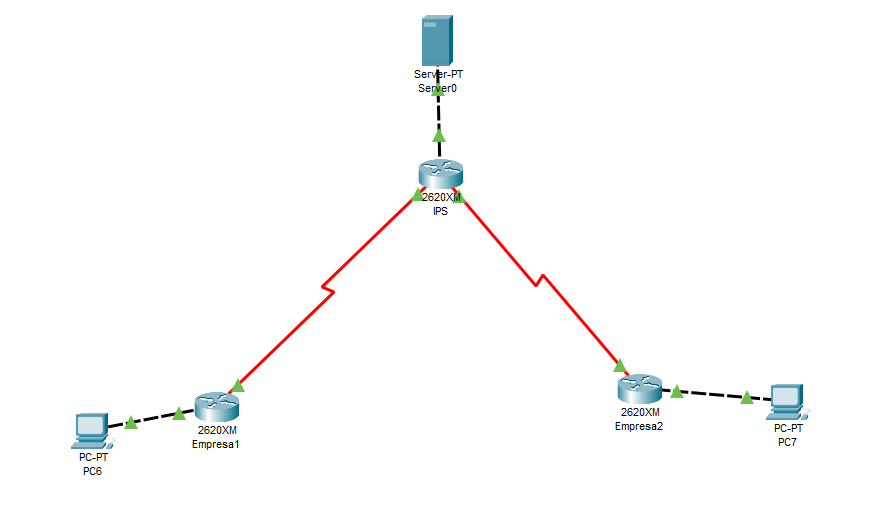
\includegraphics[width=0.7\textwidth]{img/Topologia.png}
        \caption{Topología de red}
        \label{fig:topologia}
    \end{figure}
    
    \subsection{Configuracion de los routers}
    En la imagen~\ref{fig:Imagen_Ejemplo2} se puede apreciar la configuración del router que contiene el DTE, ya que está conectado a la red del servidor que aloja la página web. En este caso, el propósito es mostrar el servidor del proveedor de servicios de Internet.
    \begin{figure}[H]
        \centering
        \includegraphics[width=0.6\textwidth]{img/2.jpg}
        \caption{Configuración del router DTE}
        \label{fig:Imagen_Ejemplo2}
    \end{figure}

    En este caso, se puede observar la IP configurada en el puerto que se conecta al servidor. La IP del servidor es 10.0.0.10, por lo que la puerta de enlace es 10.0.0.1.
    
    En la imagen~\ref{fig:Imagen_Ejemplo5} se puede apreciar la configuración del router que contiene el DCE.

    \begin{figure}[H]
        \centering
        \includegraphics[width=0.6\textwidth]{img/5.jpg}
        \caption{Configuración del router DCE}
        \label{fig:Imagen_Ejemplo5}
    \end{figure}

    En la imagen~\ref{fig:Router DCE Empresa 1} se puede apreciar la configuración del router que contiene el DCE, ya que está conectado a la red del cliente que solicita la página web. En este caso, el propósito es mostrar el cliente que solicita la página web.

    \begin{figure}[H]
        \centering
        \includegraphics[width=0.6\textwidth]{img/3.jpg}
        \caption{Configuración del router DCE}
        \label{fig:Router DCE Empresa 1}
    \end{figure}

    \subsection{configuración de los protocolos}
    En la imagen~\ref{fig:NAT empresa 1} se puede apreciar la configuración de los protocolos en el router que contiene el DCE. Se observa que solo se enrutan las redes públicas, mientras que en las redes privadas se utiliza NAT con su protocolo PAT, de manera que se pueda acceder al servidor del proveedor de servicios de Internet.
    
    \begin{figure}[H]
        \centering
        \includegraphics[width=0.6\textwidth]{img/4.jpg}
        \caption{Configuración de los protocolos}
        \label{fig:NAT empresa 1}
    \end{figure}

    En la imagen~\ref{fig:EIGRP isp} se puede apreciar la configuración del protocolo EIGRP para el proveedor de internet, en la cual se observa que se enrutan las redes públicas. Dado que no tenemos redes privadas, no es necesario enrutarlas.

    \begin{figure}[H]
        \centering
        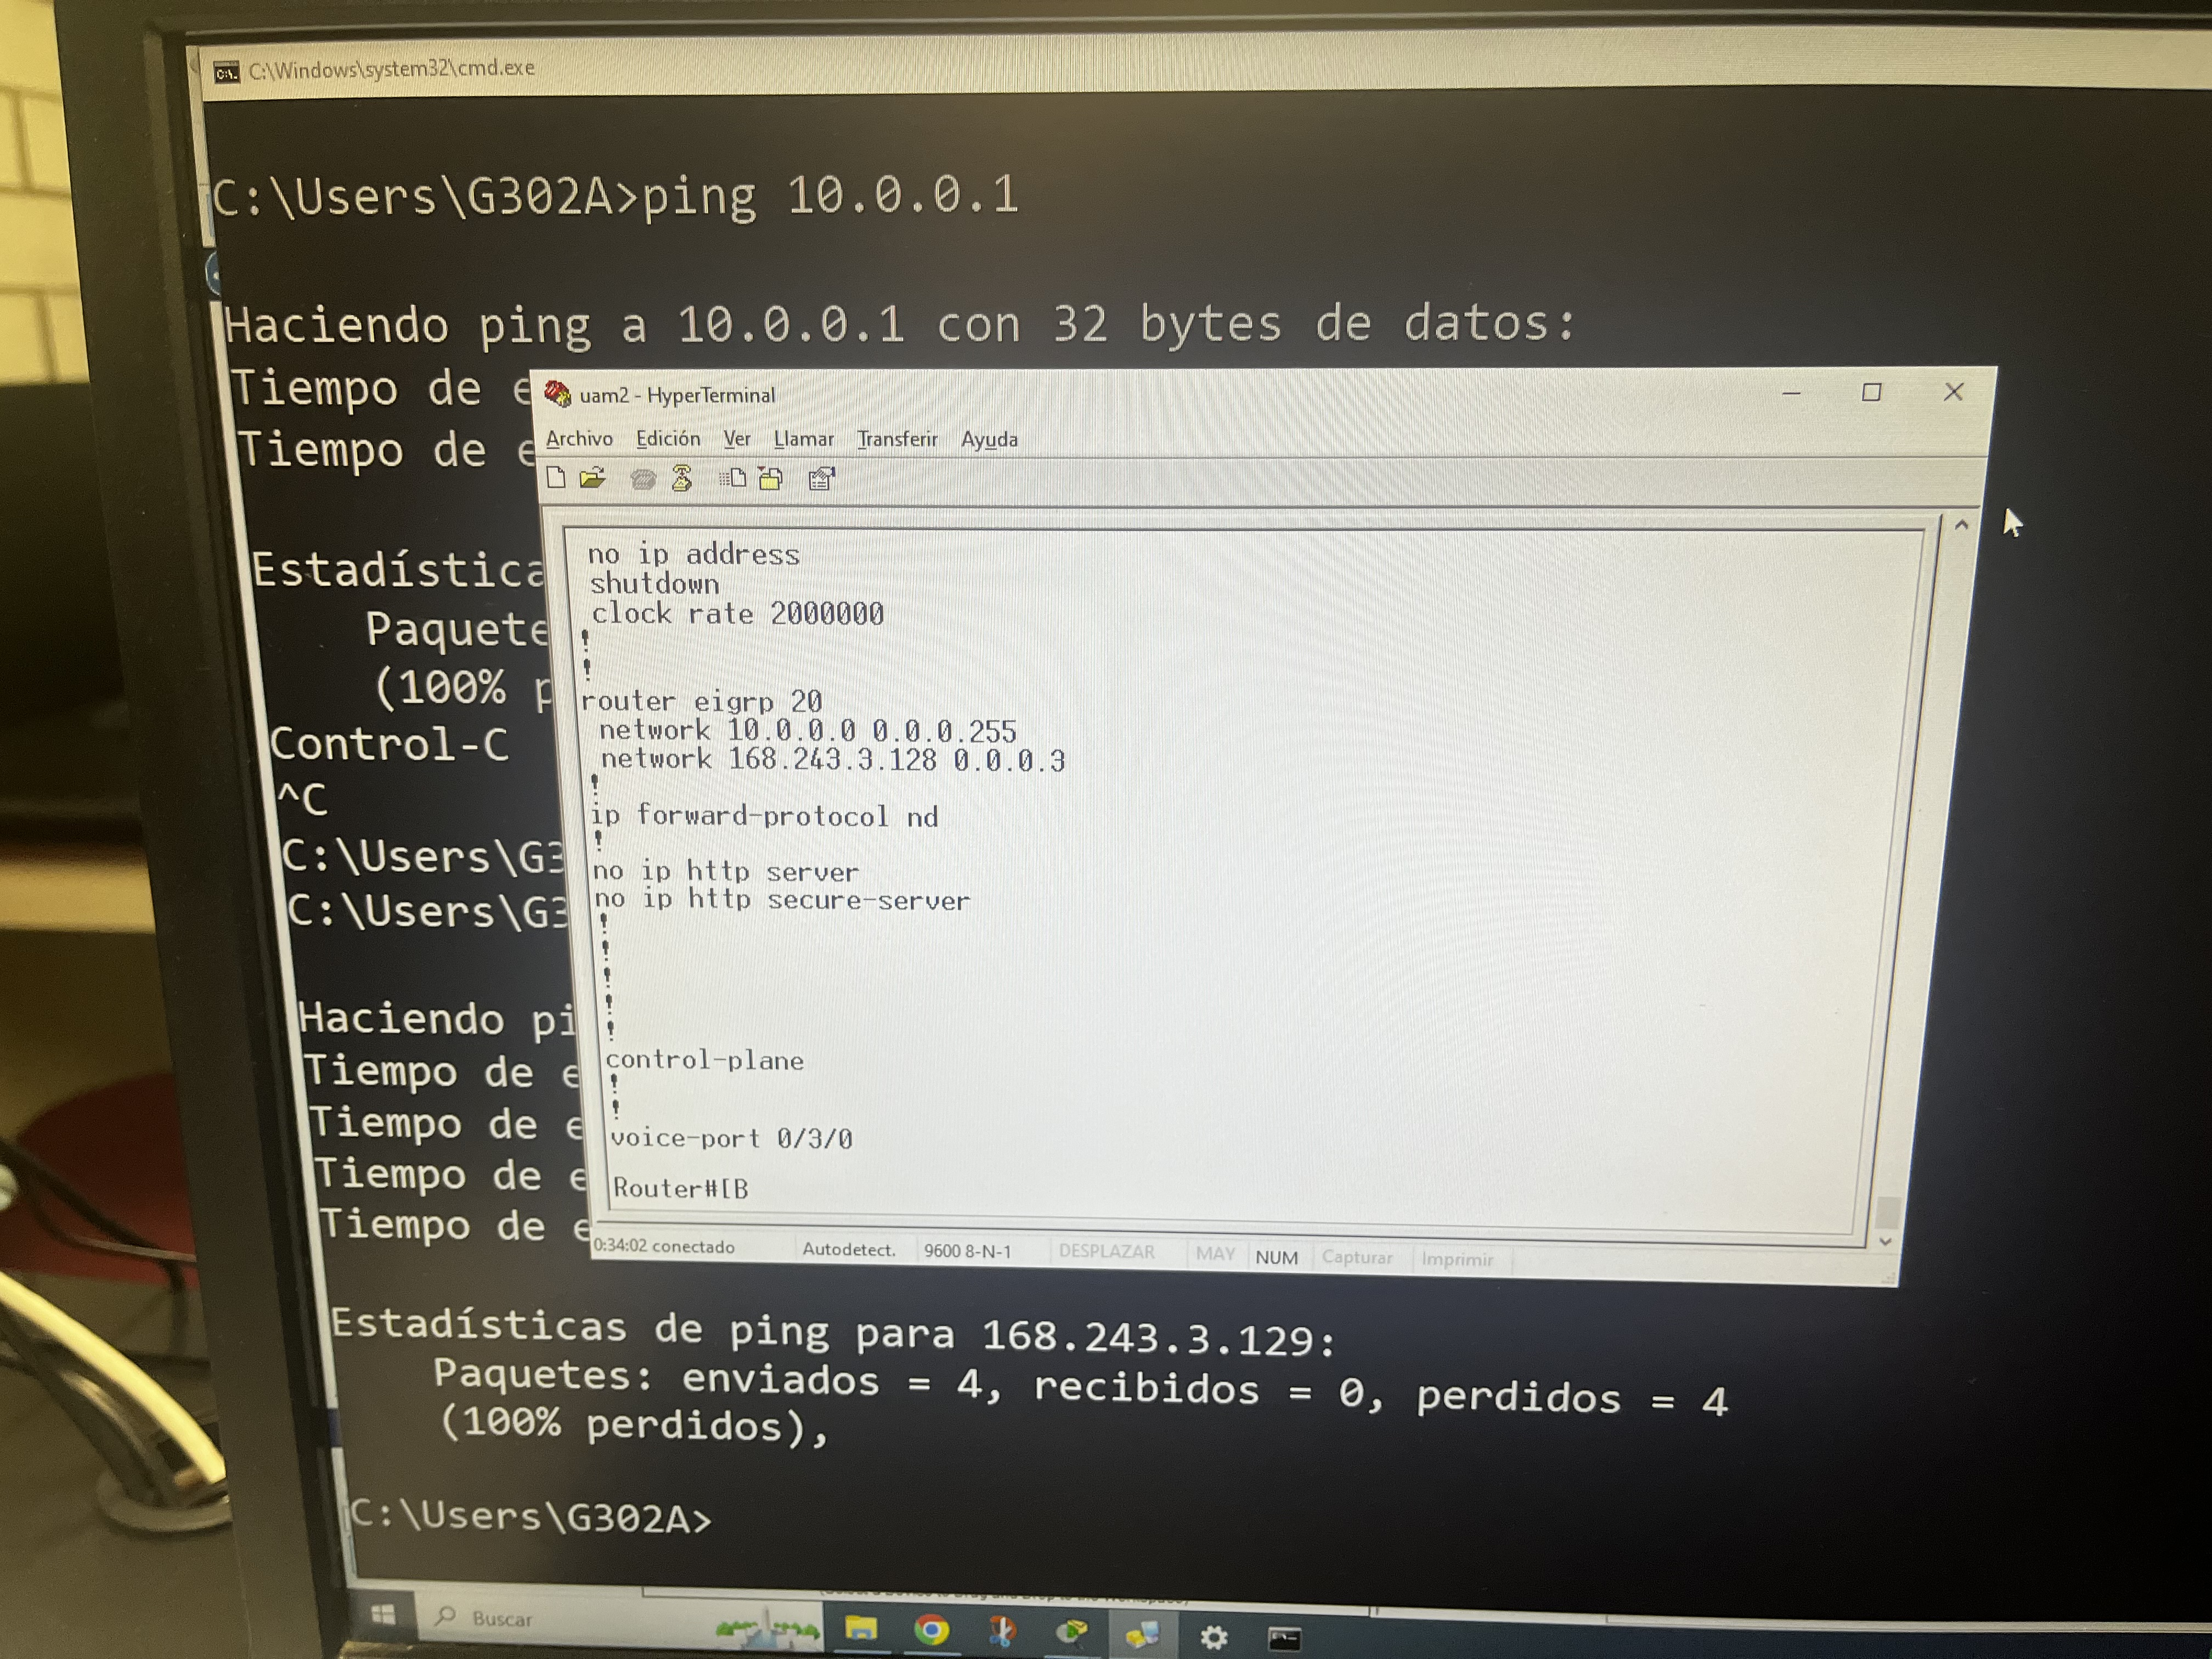
\includegraphics[width=0.6\textwidth]{img/6.jpg}
        \caption{Configuración del protocolo EIGRP}
        \label{fig:EIGRP isp}
    \end{figure}

    En la imagen~\ref{fig:Pruebas_conexion} se puede apreciar que se realizaron pruebas para la conexión al servidor del proveedor de servicios de Internet. Se puede observar que existe conexión y comunicación entre el cliente y el servidor mediante el comando ping.

    \begin{figure}[H]
        \centering
        \includegraphics[width=0.6\textwidth]{img/1.jpg}
        \caption{Pruebas de conexión}
        \label{fig:Pruebas_conexion}
    \end{figure}

\section{Conclusiones}

\begin{itemize}
    \item Diego Alexis Moreno Valero - 2243900185\\
    Se puede concluir que, debido a la falta de tiempo, no fue posible completar correctamente la práctica del laboratorio asignada, por lo que no podemos emitir una evaluación sobre los resultados obtenidos. Sin embargo, todos los comandos y las imágenes presentadas corresponden a los realizados durante la práctica.
    \item Luis Ángel Cruz Díaz - 2183038433 \\
    En esta práctica no se pudó probar el completo funcionamiento de la red debido a no tener acceso a los dispositivos de red y el poco tiempo para realizar la práctica. Sin embargo, se logró configurar los routers y los protocolos necesarios para que la red funcione correctamente.
\end{itemize}


% --- Para agregar un apéndice
%\newpage
%\appendix
%\appendixpage
%\addappheadtotoc
%\section{Nombre del apéndice}